\section{Software}
\subsection{MatrixAngle}
\label{sec:matrixAngle}
\textsl{MatrixAngle} es el Software que se ha desarrollado para gestionar la
conversión de las imágenes y animaciones, y el control remoto del sistema. A
modo de resumen exponemos estas capturas indicando el funcionamiento y las
características de la aplicación.

\begin{figure}[!ht]
	\centering

	\begin{subfigure}[t]{\textwidth}
		\centering
		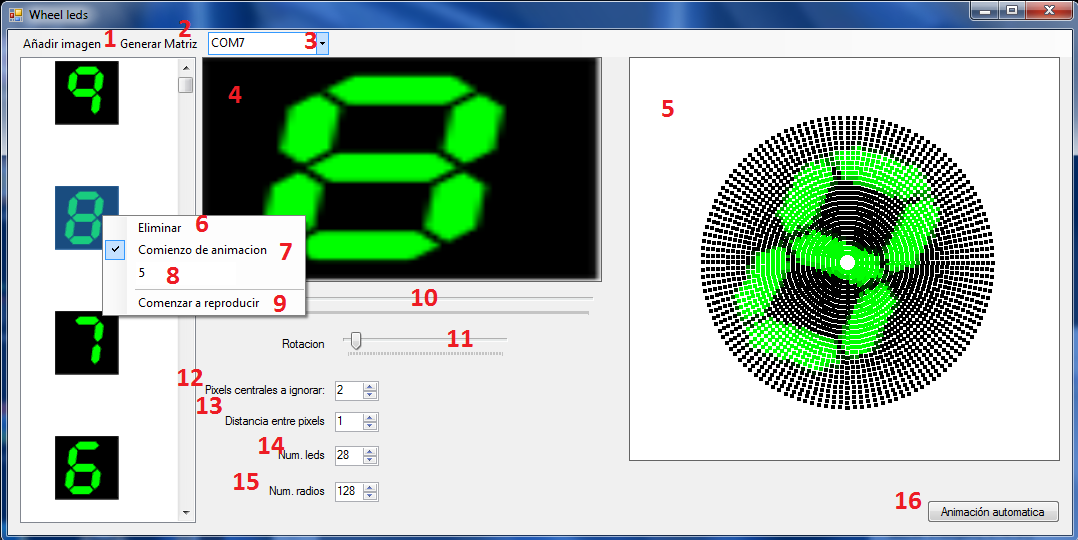
\includegraphics[width=\textwidth]{images/matrixAngle1}
		\caption{Gestión de frames y posición de imágenes en la rueda}
		\label{fig:matrixAngle1}
	\end{subfigure}
	\\
	\begin{subfigure}[b]{\textwidth}
		\centering
		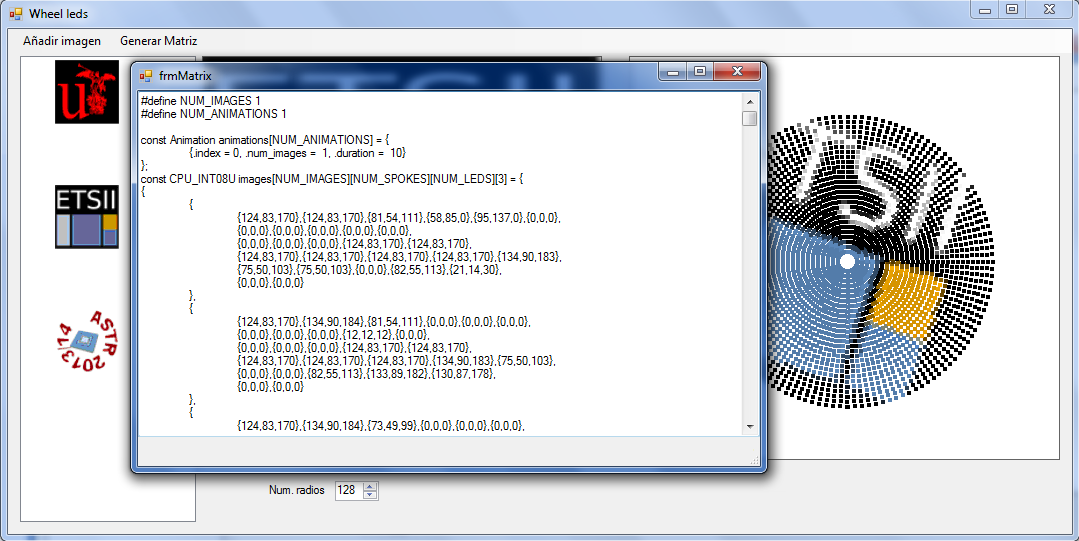
\includegraphics[width=\textwidth]{images/matrixAngle2}
		\caption{Generación del código C con la estructura de las
		imágenes convertidas y las animaciones}
		\label{fig:matrixAngle2}
	\end{subfigure}

	\caption{Imágenes que ilustran el funcionamiento y las características
	de \textsl{MatrixAngle}}
\end{figure}

Lista de características:
\begin{enumerate}
	\item Permite buscar una imagen para agregarla a la lista de frames.
	\item Genera el código C con la estructura de la matriz que contiene
		todas las imágenes seleccionadas (con el formato adecuado para
		la placa), junto con una estructura con información sobre las
		animaciones.
	\item Selecciona el puerto del FTDI por el que se transmitirán los
		comandos al sistema.
	\item Muestra la imagen seleccionada.
	\item Simulación de como se vería la imagen en la rueda.
	\item Elimina el frame seleccionado.
	\item Selecciona el frame actual como el frame de comienzo de una
		animación.
	\item Numero de repeticiones de la animación.
	\item Envía un comando al sistema para que comience a reproducir la
		animación seleccionada.
	\item Ajuste de la velocidad de simulación.
	\item Rotación de la imagen.
	\item Define el hueco central de la imagen en la rueda.
	\item Distancia entre los pixeles que se muestrean.
	\item Numero de LEDs totales en cada radio.
	\item Número de subdivisiones de la rueda.
	\item Envía el comando al sistema para que pase automáticamente de una
		animación a otra.
\end{enumerate}

\subsection{CyclePOV Emulator}
Este programa se creó para simular la carga y visualización en la rueda, de la
matriz generada por \textsl{MatrixAngle} (\refcont{sec:matrixAngle}) y así poder
solucionar algunos errores de forma más cómoda que utilizando la rueda.

\begin{figure}[!ht]
	\centering

	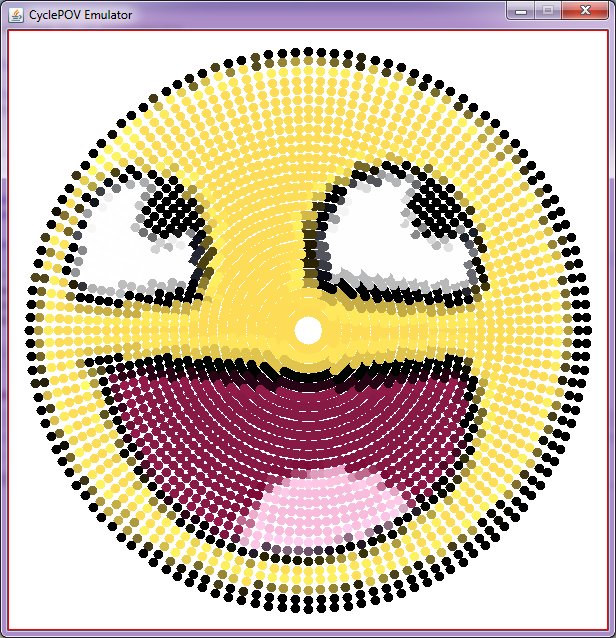
\includegraphics[width=\textwidth]{images/cyclePOVemulator}
	\caption{Captura del programa CyclePOV Emulator simulando la carga y
	visualización de una imagen.}
\end{figure}
